\chapter{最短路径算法实现}
\section{最短路径算法分析}
\par 在二维空间中,通常是基于二维垂直的欧几里得空间,其中x轴和y轴垂直,顶点通常以类似经纬度形式给出,如~(x,y)~代表该顶点分别该点坐标分别在x轴、y轴上的长度分量,点~(a,b)~在~x~轴的分量为~a~,在~y~轴的分量为~b~;其中顶点之间会与若干条路径相连,其中路径不能经过相关障碍物,路径的权值可以是该条路径的长度或该条路径所需费用,记为~W(i,j)~表示第~i~个顶点到第~j~个顶点的边的权值。例如在运输网络中,顶点代表的是不同城市的集散地,顶点之间的路径就是城市之间的交通网,路径的权值代表该条交通路线所需要的时间,则所求的顶点到顶点的最短路径即是最短时间的路线。
\subsection{基于Dijkstra算法的最短路径求解}
\par Dijkstra该算法基于贪心的思想,解决了图~G=<V,E>~上带权的单源最短路径问题,通过设置一顶点集合~S~,在集合S中所有的顶点与源点s之间的最终最短路径权值均已被计算出来。算法反复选择最短路径估计最小的点$u\in V-S$并将~u~加入到~S~中,最终计算出源点到其他所有点的最短距离。举例来说,若图中的顶点代表城市,而边上的权值表示城市间开车行车的距离,该算法可以用来找到两个城市之间的最短路径。但是Dijkstra算法并不能有效处理带有负权边的图。
\par 算法描述:Dijkstra算法通过保留目前为止所找到的每个顶点$v\in V$从~s~到~v~的最短路径来工作。初始时,原点s的路径权重被赋为0。同时把所有顶点的路径长度设为无穷大,即表示我们不知道任何通向这些顶点的路径。当算法结束后,~d[v]~中存储的便是从s到v的最短路径,或者如果路径不存在的话是无穷大。
\par 松弛操作是Dijkstra的基础操作:如果存在一条从u到v的边,那么从s到v的一条新路径是将边$w(u,v)\in E$添加到从s到u的路径尾部来拓展一条从s到v的路径。这条路径的长度是$d[u]+w(u,v)$。若这个值比目前已知的$d[v]$的值要小,那么可以用这个值来替代当前$d[v]$中的值。松弛边的操作一直运行到所有的$d[v]$都代表从s到v的最短路径的长度值。由于基于松弛操作,因此若存在负权值边中的负环时会重复松弛,导致无法正确求解出最短路径。
\par 算法维护两个顶点集合openList和clostList,集合openList保留所有已知实际最短路径值的顶点,而集合clostList则保留其他所有顶点。集合S初始状态为空,而后每一步都有一个顶点从Q移动到S。这个被选择的顶点是Q中拥有最小的$d[u]$值的顶点。当一个顶点~u~从~Q~中转移到了~S~中,算法对u的每条外接边$w(u,v)$进行松弛。
\par 算法的步骤如下
\begin{enumerate}
    \item 输入边全为正权的图,G中带有顶点V=$v_0,v_1,v_2\dots$和若干边$w(v_i,v_j)$
    \item 设置一个待检测列表clostList和一个不需检测列表clostList;
    \item 将起始点startPoint加入openList中;
    \item 初始化距离向量~d~,其中startPoint的距离为0,其他全为正无穷;
    \item 检测openList,找出~d~值最小的一个点,将此节点作为当前节点(curNode),并加入closeList中不再检测;
    \item 若该点等于终点endPoint,此时终止算法,已找到最短路径,返回该点的距离向量;
    \item 否则遍历curNode的相邻节点,若该节点是不可通过的、或在closeList中的、或超过边界的,则跳过;
    \item 保存该节点的parent为curNode,计算其距离向量值~d~,再保存到openList中;
    \item 若此时openList为空,算法结束,未找到起点到终点的最短路径;
    \item 若openList不为空,回到步骤5;
\end{enumerate}
\par 算法中的步骤8,计算相邻节点(Node)的距离向量~d~时,即是算法的松弛操作,具体计算方法是:$if (d[curNode] + w(curNode, Node) < d[Node]) d[Node] = d[curNode] + w(curNode, Node)$,通过不断的将所有点加入openList来松弛到其他顶点的距离向量,最后就能计算出从起点到终点的最短路径了。
\par 例如使用该算法来寻找两个城市之间的最短路径,整个图是城市之间的交通网,此时顶点是城市,顶点之间的路径是城市之间的交通路线,路径的权值是行驶所需的时间,因此两个城市之间可能有多条权值不同的路径,此时使用Dijkstra算法求解得到的最短路径即是从起点出发到其他顶点的所需要的最短时间的路线。
\subsection{基于A*算法的最短路径求解}
\par A*搜索算法综合了最良优先算法(Best-first search)和Dijkstra算法的优点:在进行启发式搜索提高算法效率的同时,可以保证找到一条最优路径(基于评估函数)。
\par 该算法中,以~g(n)~表示从起点到任意顶点n的实际距离,~h(n)~表示任意顶点n到目标顶点的估算距离,那么A*算法的估算函数为~f(n)=g(n)+h(n)~,这个公式遵循以下特性:
\begin{itemize}
    \item 如果~g(n)~为0,即只计算任意顶点n到目标的评估函数~h(n)~,而不计算起点到顶点n的距离,则算法转化为使用贪心策略的最良优先搜索,速度最快,但可能得不出最优解;
    \item 如果~h(n)~不大于顶点n到目标顶点的实际距离,则一定可以求出最优解,而且~h(n)~越小,需要计算的节点越多,算法效率越低,常见的评估函数有-欧几里得距离、曼哈顿距离、切比雪夫距离;
    \item 如果~h(n)~为0,即只需求出起点到任意顶点n的最短路径~g(n)~,而不计算任何评估函数~h(n)~,则转化为单源最短路径问题,即Dijkstra算法,此时需要计算最多的顶点。
\end{itemize}
\par 其步骤如下
\begin{enumerate}
    \item 设置一个待检测列表openList和一个不需检测列表clostList;
    \item 把起始点startPoint加入openList中;
    \item 检测openList,找出其中~f~值最小的一个点,将此节点作为当前节点(curNode),并加入closeList中不再检测;
    \item 若该点等于终点endPoint,此时终止算法,已找到最短路径;
    \item 否则遍历curNode周围的节点,若该节点是不可通过的、在closeList中的、超过边界的,则跳过;
    \item 保存该节点的parent,计算~f~值,再保存到openList中;
    \item 若此时openList为空,算法结束,未找到目的点;
    \item openList不为空,回到步骤3;
\end{enumerate}
\par A*算法通过启发式搜索,即评估函数~h(n)~,进一步提高了寻找最短路径的效率,减小了无用点的遍历过程,可以大大的节省时间和空间的消耗。
\section{三维最短路径}
\par 对于类似实际空间的三维空间,由于三维空间当中顶点的数量较多,且存在复杂的障碍物关系,使得在三维空间中求解最短路径算法对于空间复杂度和时间复杂度之间存在一定的受限,在三维空间当中求解最短路径更偏向于求解近似最短路径,以满足时间和空间的要求,因此算法主要解决在一定的精度误差内近似求解出给出起点到终点之间的最短路径长度及所经过的顶点路径。
假设空间离散时精度为~precision~,即代表实际空间中的1单位长度对应离散化空间的~precision~单位长度。
则在实际空间中的点坐标~(x,y,z)~可以离散化为格子点坐标$(\lfloor\dfrac{x}{precision}\rfloor,\lfloor\dfrac{y}{precision}\rfloor,\lfloor\dfrac{z}{precision}\rfloor)$,则我们需要对起点、终点和障碍物都完成离散化的过程,然后在离散化空间中求解起点到终点的最短路径。

\subsection{数据处理}
\par 首先,根据实际空间的障碍物,模型成若干个如图的长方体,其中长方体满足底面为一个矩形,但可能长宽不平行于x、y轴,高平行于三维空间的z轴。数据中会以实数给出底面矩形平行的两边的中点$M_0(a,b),M_1(c,d)$,与之垂直的边的长度~D~,以及该立方体的z轴范围$z_0,z_1$。通过给出的数据可以计算得出该长方体障碍物所对应的顶点。
根据实际空间模型,需要首先按照指定的精度将实际空间的模型划分到指定精度的空间,将空间划分为若干个离散化的格点,通过计算该精度下障碍物所经过的格子点,这些障碍物的离散格点都是在计算最短路径时不可以通过的。
\par 根据障碍物底面为一个矩形,其满足长与宽垂直,则设两中点$M_0,M_1$所在直线为矩形的长,则如图\ref{fig:obstacle_bottom},设该矩形的四个顶点分别为$A(x_0,y_0)$、$B(x_1,y_1)$、$C(x_2,y_2)$、$D(x_3,y_3)$且满足相邻的关系,则有$\vec{M_0A}\times\vec{M_0M_1}=0$,根据$M_0M_1$直线的表达式,可以计算出直线$M_0A$的表达式,且矩形的宽为~D~,则$d(M_0,A)=\frac{D}{2}$,故有$\sqrt{(a-x_0)^2+(b-y_0)^2}=\frac{D}{2}$。
联系上述两方程,可以得到与$M_0$相邻的顶点的坐标分别为$$A=\dfrac{x_0}{2}$$特别注意特殊判断长宽平行与轴的情况,即四个顶点的坐标为$$$$。
具体的代码如图\ref{fig:3axis},通过if-else判断情况来具体计算,最后使用结构体存储,方便后续使用。
\par 通过处理数据,使得可以将最短路径算法应用在三维空间当中,通过控制离散化的精度来实现控制最短路径的精度,离散后格点的标记来实现不可访问情况的判断,达到将实际空间离散化到指定精度的理想空间,从而计算出格点组成的最短路径。
\begin{figure}[h]
    \centering
    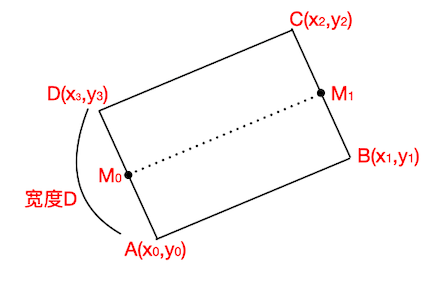
\includegraphics[width=12cm]{figures/obstacle_bottom.png}
    \caption{障碍物底面}
    \label{fig:obstacle_bottom}
\end{figure}

\subsection{相交判断}
\par 通过计算出格点组成的最短路径后,由于存在三角形定则,即三角形两边之和大于第三边,所以在计算的格点路径后,是可以通过运用三角形定则拟合计算出更短的路径,此时就需要判断所拟合的新路径是否经过了障碍物。此时问题可以抽象为线段与长方体是否相交的判定问题,根据线段的向量表示法,有线段PQ:$P+k(Q-P),k\in [0,1]$,若存在与某个障碍物相交的情况,即存在k属于0~1之间,使得该点在障碍物之内。设该点坐标为$(x,y,z)$

\subsection{最短路径算法}
\subsubsection{基于BFS的最短路径算法}
\subsubsection{基于A*的最短路径算法}
\subsection{实例}

\section{本章总结}
